\documentclass[a4paper, openany, UTF8]{ctexbook}

\usepackage{asymptote}
\usepackage{amsmath}
\usepackage{amssymb}
\usepackage{amsthm}
\usepackage{float}
\usepackage{geometry}
\usepackage{graphicx}
\usepackage[colorlinks=true]{hyperref}
\usepackage[toc]{multitoc}
\usepackage{paralist}
\usepackage{subcaption}
\usepackage{ulem}
\usepackage{wrapfig2}
\usepackage{xcolor}

\setlength{\parskip}{1ex plus 0.5ex minus 0.2ex}
\geometry{inner=1in,outer=1.25in}

\newtheorem{axiom}{公理}[chapter]
\newtheorem{corollary}{推论}[chapter]
\newtheorem{example}{例}[section]
\newtheorem{lexample}{引例}[chapter]
\newtheorem{theorem}{定理}[chapter]

\let\enumerate\compactenum
\let\endenumerate\endcompactenum
\let\itemize\compactitem
\let\enditemize\endcompactitem

\title{{\Huge 高中数学笔记}}
\author{郑}

\begin{document}
	\begin{asydef}
		import settings;
		batchMask = false;
		interactiveMask = true;
		batchView = false;
		interactiveView = true;
		prc = false;
	\end{asydef}

	\frontmatter
	\setcounter{tocdepth}{1}
	\maketitle

	\section*{前言}
简而言之,该数学笔记整理了高中数学的所有知识点,供各位同学参考. 它有点像教科书,但又不是教科书,这一点会在正文中慢慢体现出来.

这本笔记分成了如下部分:

\begin{description}
	\item[代数] 包含方程与不等式、最值值域和恒成立与有解等内容
	\item[函数] 涵盖了函数图像、单调性、对称性、周期性以及导数
	\item[向量和复数] 向量和复数的相关知识
	\item[立体几何] 主要讲述以向量解决立体几何问题
	\item[计数原理] 排列组合和二项式的知识
\end{description}

该数学笔记亦提供了计算器的使用说明,适用于卡西欧\verb|fx-991CN X|.

这本笔记是开源的,您可以在\href{https://github.com/jason-bowen-zheng/math-notes}{这里}获取全部的源代码,亦可以提出改进意见.
\hypersetup{hidelinks}

\begin{flushright}
	\date{2022年11月}于上海
\end{flushright}


	\tableofcontents
	\clearpage
	\mainmatter
	\raggedbottom

	\part{函数}
	\chapter{导数}
在此首先恭喜您,当看到“导数”这个词时,阁下即将面对的是数学的一个全新的分支---\textbf{微积分学}(calculus)。简而言之,它将我们研究函数的视角从宏观拓展到了微观。

听起来似乎很难,不过这只是高中难度的知识,我们也只学习导数及其应用,也没这么难吧(应该)。

YouTube频道3Blue1Brown有10部讲述“微积分的本质”的视频,我会按学习进度推荐您看其中的6部。

\section{概念}
有一描述直线的函数$f(x)=2x$,当问及“$x=1$时函数的斜率是多少”,您一定会说是2。这很简单,因为$f(x)$的斜率处处相等。

那请问当$x=1$时,$f(x)=x^2$的斜率为多少呢?

作为一个不知道微积分为何物的高中生,您决定试一试,透过斜率的定义\footnote{简单来说,斜率$k=\dfrac{\Delta y}{\Delta x}$,即垂直方向的变化量与水平方向的变化量的比值。}来解决这个问题。

\begin{figure}[htb]
    \centering
    \begin{asy}
        import graph;
        write("asy: Generating 'fig:calc-slope'");

        size(4cm, 4cm);

        real f(real x){return x^2;}
        real fp(real x){return 2.5*x-1.5;}

        draw(graph(f, -2, 2), red);
        draw(graph(fp, 0, 2), blue);
        xaxis("$x$", EndArrow);
        yaxis("$y$", EndArrow);

        draw((1, 1) -- (1.5, 1), L=scale(0.5)*Label("$\Delta x$", position=MidPoint));
        draw((1.5, 1) -- (1.5, 1.5^2), L=scale(0.5)*Label("$\Delta y$", position=MidPoint));
        dot((1, 1), L=scale(0.5)*Label("$A$", align=NW));
        dot((1.5, 1.5^2), L=scale(0.5)*Label("$B$", align=W));
    \end{asy}
    \caption{计算二次函数的斜率}
    \label{fig:calc-slope}
\end{figure}

您或许会画出如图\ref{fig:calc-slope}所示的函数图像,那接下来我们就可以使用由两条直角边$\Delta x$和$\Delta y$组成的直角三角形来计算斜率。

二次函数上$A$点处的斜率是我们要求的,我们可以让抛物线上的$B$点慢慢靠近$A$点,这样直角三角形会越来越小,结果也会变得精确。我们就可以写出式子\eqref{equ:calc-slope}来表示斜率
\begin{gather}
    k=\frac{(1+\Delta x)^2-1^2}{\Delta x} \label{equ:calc-slope}
\end{gather}

给$\Delta x$多次赋值,我们不难发现最后它会收敛到2,由此可知$f(x)=x^2$在$x=1$处的斜率是2。
\begin{align*}
    \Delta x=0.1\quad & k=2.1 \\
    \Delta x=0.01\quad & k=2.01 \\
    \Delta x=0.001\quad & k=2.001 \\
\end{align*}

好,我们算完了,感觉很简单吧!\textbf{导数}(derivative)就是这样,研究函数在某一点附近的变化率。我们刚刚寻找函数某点导数的过程称为\textbf{求导}(differentiation)。

同时,为了避免每次求导都要考虑函数图像,求$f(x)$在$x=x_0$处的导数$f'(x_0)$有公式\[f'(x_0)=\lim_{h\to0}\frac{f(x_0+h)-f(x_0)}{h}\]这和我们刚刚得到的式子\eqref{equ:calc-slope}很像,只不过我们使用了极限的表示方法。

% TODO: \section{公式}
% TODO: \section{运用}


	\part{三角学}
	\chapter{三角比}
在初中时期,我们通过直角三角形定义并明白了锐角三角比。现在,我们将要学习任意角的三角比。

\section{概念}

\subsection{弧度制}
在之前很长一段时间,我们使用的都是角度制,它将一个周角分为了360等分,不过继续运用角度制会显得不够简洁。所以我们引入了\textbf{弧度}(radian),它认为一个周角是$2\pi$弧度。

从角度制转换为弧度制很简单,乘以$\dfrac{\pi}{180}$即可;以弧度表示角度,则乘以$\dfrac{180}{\pi}$,由此可知$1\mathrm{rad}=57.296^\circ$。

弧度的单位写作$\mathrm{rad}$,不过通常不写单位。

\subsection{三角比的定义}
我们用如图\ref{fig:unit-circle}的单位圆来定义任意角的三角比。虽然我们放弃了使用直角三角形定义三角比,但图中绿色部分仍然是一个三角形,只不过两条直角边(蓝边、红边)是要考虑正负的。

\begin{figure}[htb]
	\centering
    \begin{asy}
        write("asy: Generating 'fig:unit-circle'");
        size(6cm, 6cm);

        draw((-1.2, 0) -- (1.2, 0), Arrow, L=Label("$x$", position=EndPoint));
        draw((0, -1.2) -- (0, 1.2), Arrow, L=Label("$y$", position=EndPoint));
        draw(unitcircle);
        draw((0, 0) -- (1/2, sqrt(3)/2), linewidth(1.5), L=Label("$r$", position=MidPoint, align=N));
        fill((0, 0) -- (1/2, 0) -- (1/2, sqrt(3)/2) -- cycle, palegreen);
        draw((0, 0) -- (0.5, 0), blue+1);
        draw((1/2, 0) -- (1/2, sqrt(3)/2), red+1);
        draw(arc((0, 0), r=0.3, angle1=0, angle2=60), arrow=Arrow(TeXHead), L=Label("$\theta$", position=Relative(0.3), align=W));

        label("$P$", (1/2, sqrt(3)/2), align=NE);
    \end{asy}
	\caption{单位圆}
	\label{fig:unit-circle}
\end{figure}

与锐角三角比类似,我们可以定义终边$r$与$x$轴正半轴夹角$\theta$的三角比
\begin{align*}
    \sin\theta=\frac{y}{r}\quad & \cos\theta=\frac{x}{r} \\
    \tan\theta=\frac{y}{x}\quad & \cot\theta=\frac{x}{y} \\
    \sec\theta=\frac{r}{y}\quad & \csc\theta=\frac{r}{x}
\end{align*}

不难看出,当$r=1$时,红线的长度即$\theta$角的正弦值,称为\textbf{正弦线};同样,蓝线的长度是$\theta$角的余弦值,为\textbf{余弦线}。

所以,圆周上一点$P$可表示为\[P(r\cos\theta,r\sin\theta)\]

至于各个特殊角的三角比的值嘛,也是可以轻易算出来的,限于篇幅就不放在这里了,反正各位的教科书上也是有的。

\section{公式}
在以下4个小节中,我们将了解4类在三角学中很有用的公式(你我肯定有同感:“这玩意真多啊”,不过就20几个嘛,背就完事了)。

“三角比”和“三角函数”没有什么本质差别,所以这里直接懒得管了,将三角比和三角函数混用,请不要介意。

\subsection{变名公式}
当角度不变,只改变三角比的名称时,应该使用这组公式。

第一部分由3个含平方的等式构成
\begin{gather}
	\sin^2\alpha+\cos^2\alpha=1 \label{equ:trig-1} \\
	\tan^2\alpha+1=\sec^2\alpha \label{equ:trig-2}\\
	1+\cot^2\alpha=\csc^2\alpha \label{equ:trig-3}
\end{gather}

第二部分由4个分式组成
\begin{gather}
	\tan\alpha=\frac{\sin\alpha}{\cos\alpha} \label{equ:trig-4} \\
	\cot\alpha=\frac{1}{\tan\alpha} \label{equ:trig-5} \\
	\sec\alpha=\frac{1}{\cos\alpha} \label{equ:trig-6} \\
	\csc\alpha=\frac{1}{\sin\alpha} \label{equ:trig-7}
\end{gather}

使用以上公式要考虑结果的正负,我们也可以使用直角三角形变名。

\subsection{变角公式}
变角公式有如下常用的5类(“看到这么多公式不想背”的心情我能理解,不过这玩意不背三角学可是学不下去的)。

\paragraph{和差角公式}
$\sin$和$\cos$的和差角公式是最基础的,以下所有公式都由它俩推得
\begin{gather}
	\sin(\alpha\pm\beta)=\sin\alpha\cos\beta\pm\cos\alpha\sin\beta \label{equ:trig-8} \\
	\cos(\alpha\pm\beta)=\cos\alpha\cos\beta\mp\sin\alpha\sin\beta \label{equ:trig-9}
\end{gather}
用式子\eqref{equ:trig-8}除以式子\eqref{equ:trig-9},每项同除$\cos\alpha\cos\beta$,可得到$\tan$的和差角公式
\begin{gather}
	\tan(\alpha\pm\beta)=\frac{\tan\alpha\pm\tan\beta}{1\mp\tan\alpha\tan\beta} \label{equ:trig-10}
\end{gather}

\paragraph{倍角公式}
通过将和差角公式中的$\alpha\pm\beta$替换成$\alpha+\alpha=2\alpha$,可得到倍角公式
\begin{gather}
    \sin2\alpha=2\sin\alpha\cos\alpha \label{equ:trig-11} \\
    \cos2\alpha=\cos^2\alpha-\sin^2\alpha=2\cos^2\alpha-1=1-2\sin^2\alpha \label{equ:trig-12} \\
    \tan2\alpha=\frac{2\tan\alpha}{1-\tan^2\alpha} \label{equ:trig-13}
\end{gather}
公式\eqref{equ:trig-12}的三连等是通过公式\eqref{equ:trig-1}得来的。

\paragraph{降幂公式}
降幂公式通过倍角公式\eqref{equ:trig-11}和\eqref{equ:trig-12}得到
\begin{gather}
    \sin\alpha\cos\alpha=\frac{1}{2}\sin2\alpha \label{equ:trig-14} \\
    \sin^2\alpha=\frac{1-\cos2\alpha}{2} \label{equ:trig-15} \\
    \cos^2\alpha=\frac{1+\cos2\alpha}{2} \label{equ:trig-16}
\end{gather}

\paragraph{半角公式}
通过给降幂公式代入$\dfrac{\alpha}{2}$并开根,即可得到半角公式
\begin{gather}
    \sin\frac{\alpha}{2}=\pm\sqrt{\frac{1-\cos\alpha}{2}} \label{equ:trig-17} \\
    \cos\frac{\alpha}{2}=\pm\sqrt{\frac{1+\cos\alpha}{2}} \label{equ:trig-18} \\
    \tan\frac{\alpha}{2}=\pm\sqrt{\frac{1+\cos\alpha}{1-\cos\alpha}}=\frac{\sin\alpha}{1+\cos\alpha}=\frac{1-\cos\alpha}{\sin\alpha} \label{equ:trig-19}
\end{gather}
公式\eqref{equ:trig-19}可巧记为“$\sin$在一边,母加子减”。

\paragraph{万能公式}
也叫\textbf{正切半角公式}(tangent half-angle formula),它将函数名都统一为$\tan$且角都统一成$\dfrac{\alpha}{2}$
\begin{gather}
    \tan\frac{\alpha}{2}=\frac{2\tan\frac{\alpha}{2}}{1-\tan^2\frac{\alpha}{2}} \label{equ:trig-20} \\
    \sin\frac{\alpha}{2}=\frac{2\tan\frac{\alpha}{2}}{1+\tan^2\frac{\alpha}{2}} \label{equ:trig-21} \\
    \cos\frac{\alpha}{2}=\frac{1-\tan^2\frac{\alpha}{2}}{1+\tan^2\frac{\alpha}{2}} \label{equ:trig-22}
\end{gather}
“万能公式”当然很有用,只不过在高中时期还没有显现它的价值罢了。

% TODO: \subsection{诱导公式}

\subsection{辅助角公式}
这个公式也是非常重要的,对于正弦函数和余弦函数的线性组合,有\[a\sin x+b\cos x=\sqrt{a^2+b^2}\sin(x+\varphi)\quad(a>0)\]

其中\[\varphi=\arctan\frac{b}{a}\]

对于$a<0$的情况,$\varphi=\arctan\dfrac{b}{a}\pm\pi$(加还是减随意,不想看到$\pi$的话在根号前添负号也可以)。

% TODO: \section{化简}

	\chapter{三角函数}

	\part{计数原理}
	\chapter{计数原理}
在“计数原理”这一章节中,我们主要学习数数。不过之前我们使用的是穷举法,这实在是太麻烦了。所以我们引入了乘法原理和加法原理两种基本的计数原理,并且使用排列组合来选和/或排数量众多的元素,最后总结了常见的题型。

\section[乘法原理]{乘法原理(分步)}
\textbf{乘法原理}(rule of product或multiplication principle)简而言之是“完成一件事要依次完成$n$个步骤,第一步有$a_1$种方法,第二步有$a_2$种方法,$\dots$,第$n$步有$a_n$种方法,则完成这件事共有$a_1\times a_2 \times\cdots\times a_n$种方法”。

\section[加法原理]{加法原理(分类)}
与乘法原理不同,\textbf{加法原理}(rule of sum或addition principle)是“完成一件事有$n$类不同的方法,第一类有$a_1$种方法,第二类有$a_2$种方法,$\dots$,第$n$类有$a_n$种方法,则完成这件事共有$a_1+a_2+\cdots+a_n$种方法”。

虽然乘法原理和加法原理的叙述很像,但它们是本质不同的两种方法:乘法原理的每一步(一个乘数)是一个步骤,整件事并没有完成;加法原理的每一类(一个加数)是完成这件事的方法数,整件事已经完成。

所以加法原理可以看作是我们使用乘法原理计算发现前步的选择对后步的可能性种数产生影响时,对各种情况进行分类讨论的一种方法

\subsection{容斥原理}
\textbf{容斥原理}(inclusion–exclusion principle)则可以看作是加法原理的拓展

\section{排列数和组合数}
在计算可能性种数的时候,与$10\times 9\times 8$类似的运算重复出现。如果相乘的数字增加,式子会变得越来越长,我们需要一种方法来简化表示方法。

因此,我们引入\textbf{排列数}(permutation),表示从$m$个元素中有顺序地选出$n$个元素的可能性种数,记作$P_m^n$,计算它的公式为\[P_m^n=\frac{m!}{(m-n)!}\]其中$n!$表示$n$的\textbf{阶乘}(factorial),表示所有小于等于该数的正整数的积,如$5!=5\times 4\times 3\times 2\times 1=120$,同时规定$0!=1$。

为了简化表示,以下的写法是等价的,这被称为“$n$的全排”。\[P_n^n=P_n=n!\]

从$m$个元素中取出(并不排序)$n$个元素称为\textbf{组合数}(combination),记作$C_m^n$,具体的公式为\[C_m^n=\frac{m!}{n!(m-n)!}\]

根据排列数的概念,$P_m^n$可写成$C_m^nP_n$,而$C_m^n$是$\dfrac{P_m^n}{n!}$

同时,对于排列数来说还有几个有用的公式
\begin{gather}
	C_n^r=C_n^{n-r} \label{equ:comb-1} \\
	C_n^0+C_n^1+\cdots+C_n^n=2^n \label{equ:comb-2} \\
	C_m^n+C_m^{n+1}=C_{m+1}^{n+1} \label{equ:comb-3}
\end{gather}
公式\eqref{equ:comb-1}可以理解为“从10个元素中取4个元素”与“从10个元素中留下6个元素”的可能性种数是相等的;而公式\eqref{equ:comb-3}可简记为“下加一,上取大”。

\begin{example}
	$C_n^3+C_n^4=C_{n+1}^6$,且$n\geq5$,求$n$。
\end{example}

\begin{proof}[解]
	可先用公式\eqref{equ:comb-3}变形为\[C_{n+1}^4=C_{n+1}^6\]

	可以套用公式\eqref{equ:comb-1}得方程\[n+1=4+6\]

	解得\[n=9\qedhere\]
\end{proof}

\section{常见题型}
最基本的计数原理也就是乘法原理和加法原理两个,灵活运用它们即可解决所有问题.不过对于某些有着典型特征的题目,这里也总结了做法。

\subsection{打包法}
我们时常会看到类似于“$\dots$要在一起”这样的要求,这个时候我们要将可以在一起的元素看成一整个元素进行排列。

\begin{example}
	$3$名男生和$4$名女生排队,女生要排在一起,问有多少种排法?
\end{example}

\subsection{插入法}
有时候也会出现“$\dots$不能在一起”的奇葩限制,我们也可以使用打包法将无限制元素打包,再将不能在一起的元素插入包中元素。

\begin{example}
	$3$名女生和$4$名男生排队,女生不能排在一起,问有多少种排法?
\end{example}

\begin{proof}[解]
	如题,“女生不能排在一起”的最简单的方法就是先排男生,然后将女生插入男生之间的空位中。

	\begin{itemize}
		\item 先找插入位,有$C_5^3$种可能
		\item 再排序要插入的元素(女生),有$P_3$种可能
		\item 最后排无限制的元素(男生),有$P_4$种可能
	\end{itemize}

	故一共有$C_5^3P_3P_4=1440$种排法。
\end{proof}

更有甚者,会有“甲、乙、丙三人中的两人可以排在一起但是三人不能同时排在一起”的类似“修罗场”的关系,也可以使用插入法解决。

\begin{example}
	$6$人排队,甲、乙、丙三人中的两人可以排在一起但是三人不能同时排在一起,问有多少种排法?
\end{example}

\subsection{插板法}
在另一些情况下我们被要求“将一些\uline{相同的}物件分给几个人,一个人\uline{至少}分到一个”,可使用\textbf{插板法}(stars and bars)来解决。

有5个相同的元素,要将其分成3组,可看成在4个空位选2个插入两块板子得到三组,即$C_4^2$种分法。

根据此种方法,将$m$个相同的元素分成$n$组,且必须分完、不出现空组的分法有\[C_{m-1}^{n-1}\]

如果允许出现空组的话,我们可以加上组数个元素再插板,被分到一个实际上是什么也没有. 这样共有$C_{m+n-1}^{n-1}$种分法。

\subsection{至多至少问题}

\subsection{混合分组}

\section[概率]{计数原理在古典概率中的应用}

	\chapter{二项式定理}
相比于之前的乘法原理和加法原理,\textbf{二项式定理}(binomial theorem)比较简单,它主要研究形如$(a+b)^n$的展开问题。

\section{公式}
我们可以先从像引例\ref{lexpl:binomial-theorem}这样简单的问题开始思考起来。

\begin{lexample}\label{lexpl:binomial-theorem}
	$(a_1+b_1)(a_2+b_2)(a_3+b_3)$的展开式是什么?
\end{lexample}

\begin{proof}[解]
	很简单,将其展开共有8项,可得(这里省略一部分)\[a_1a_2a_3+a_1a_2b_3+a_1b_2a_3+\cdots+b_1b_2b_3\qedhere\]
\end{proof}

这样的展开是很有规律的,即在每一项中,1,2,3这3个下标都出现但只出现一次,不可能出现$a_1a_2b_2$的情况。

这虽然是个简单的代数问题,但当指数处再增大一些,就麻烦了。那我们何不变化思路,将其变成一个排列组合的问题?

以$(a+b)^3$为例,每一项都是3个数相乘,即我们要从3个括号中的每一个括号里各选一个数组成一项,共有$a^3,a^2b,ab^2,b^2$这4项,每项的系数则可以看作是从$n$个$a$(或$n$个$b$)中选$k$个有多少种选法。

所以,我们可以总结二项式$(a+b)^n$展开的通项公式\[T_{r+1}=C_n^ra^{n-r}b^r=C_n^ra^rb^{n-r}\]其中,$r$可以从0取到$n$. 这里的$C_n^r$叫作每一项的\textbf{二项式系数}(binomial coefficients)。

如果对通项公式中$a$和$b$的指数可以互换感到奇怪,可以回顾公式\eqref{equ:comb-1},这无非就是将展开式颠倒了罢了。

另外,我们也可以使用如图\ref{fig:pascals-triangle}的\textbf{杨辉三角形}或\textbf{帕斯卡三角形}(Pascal's triangle)来得到二项式系数。例如:第4行对应的二项式的指数是3,对应项的二项式系数是1,3,3,1。

\begin{figure}[htb]
	\centering
	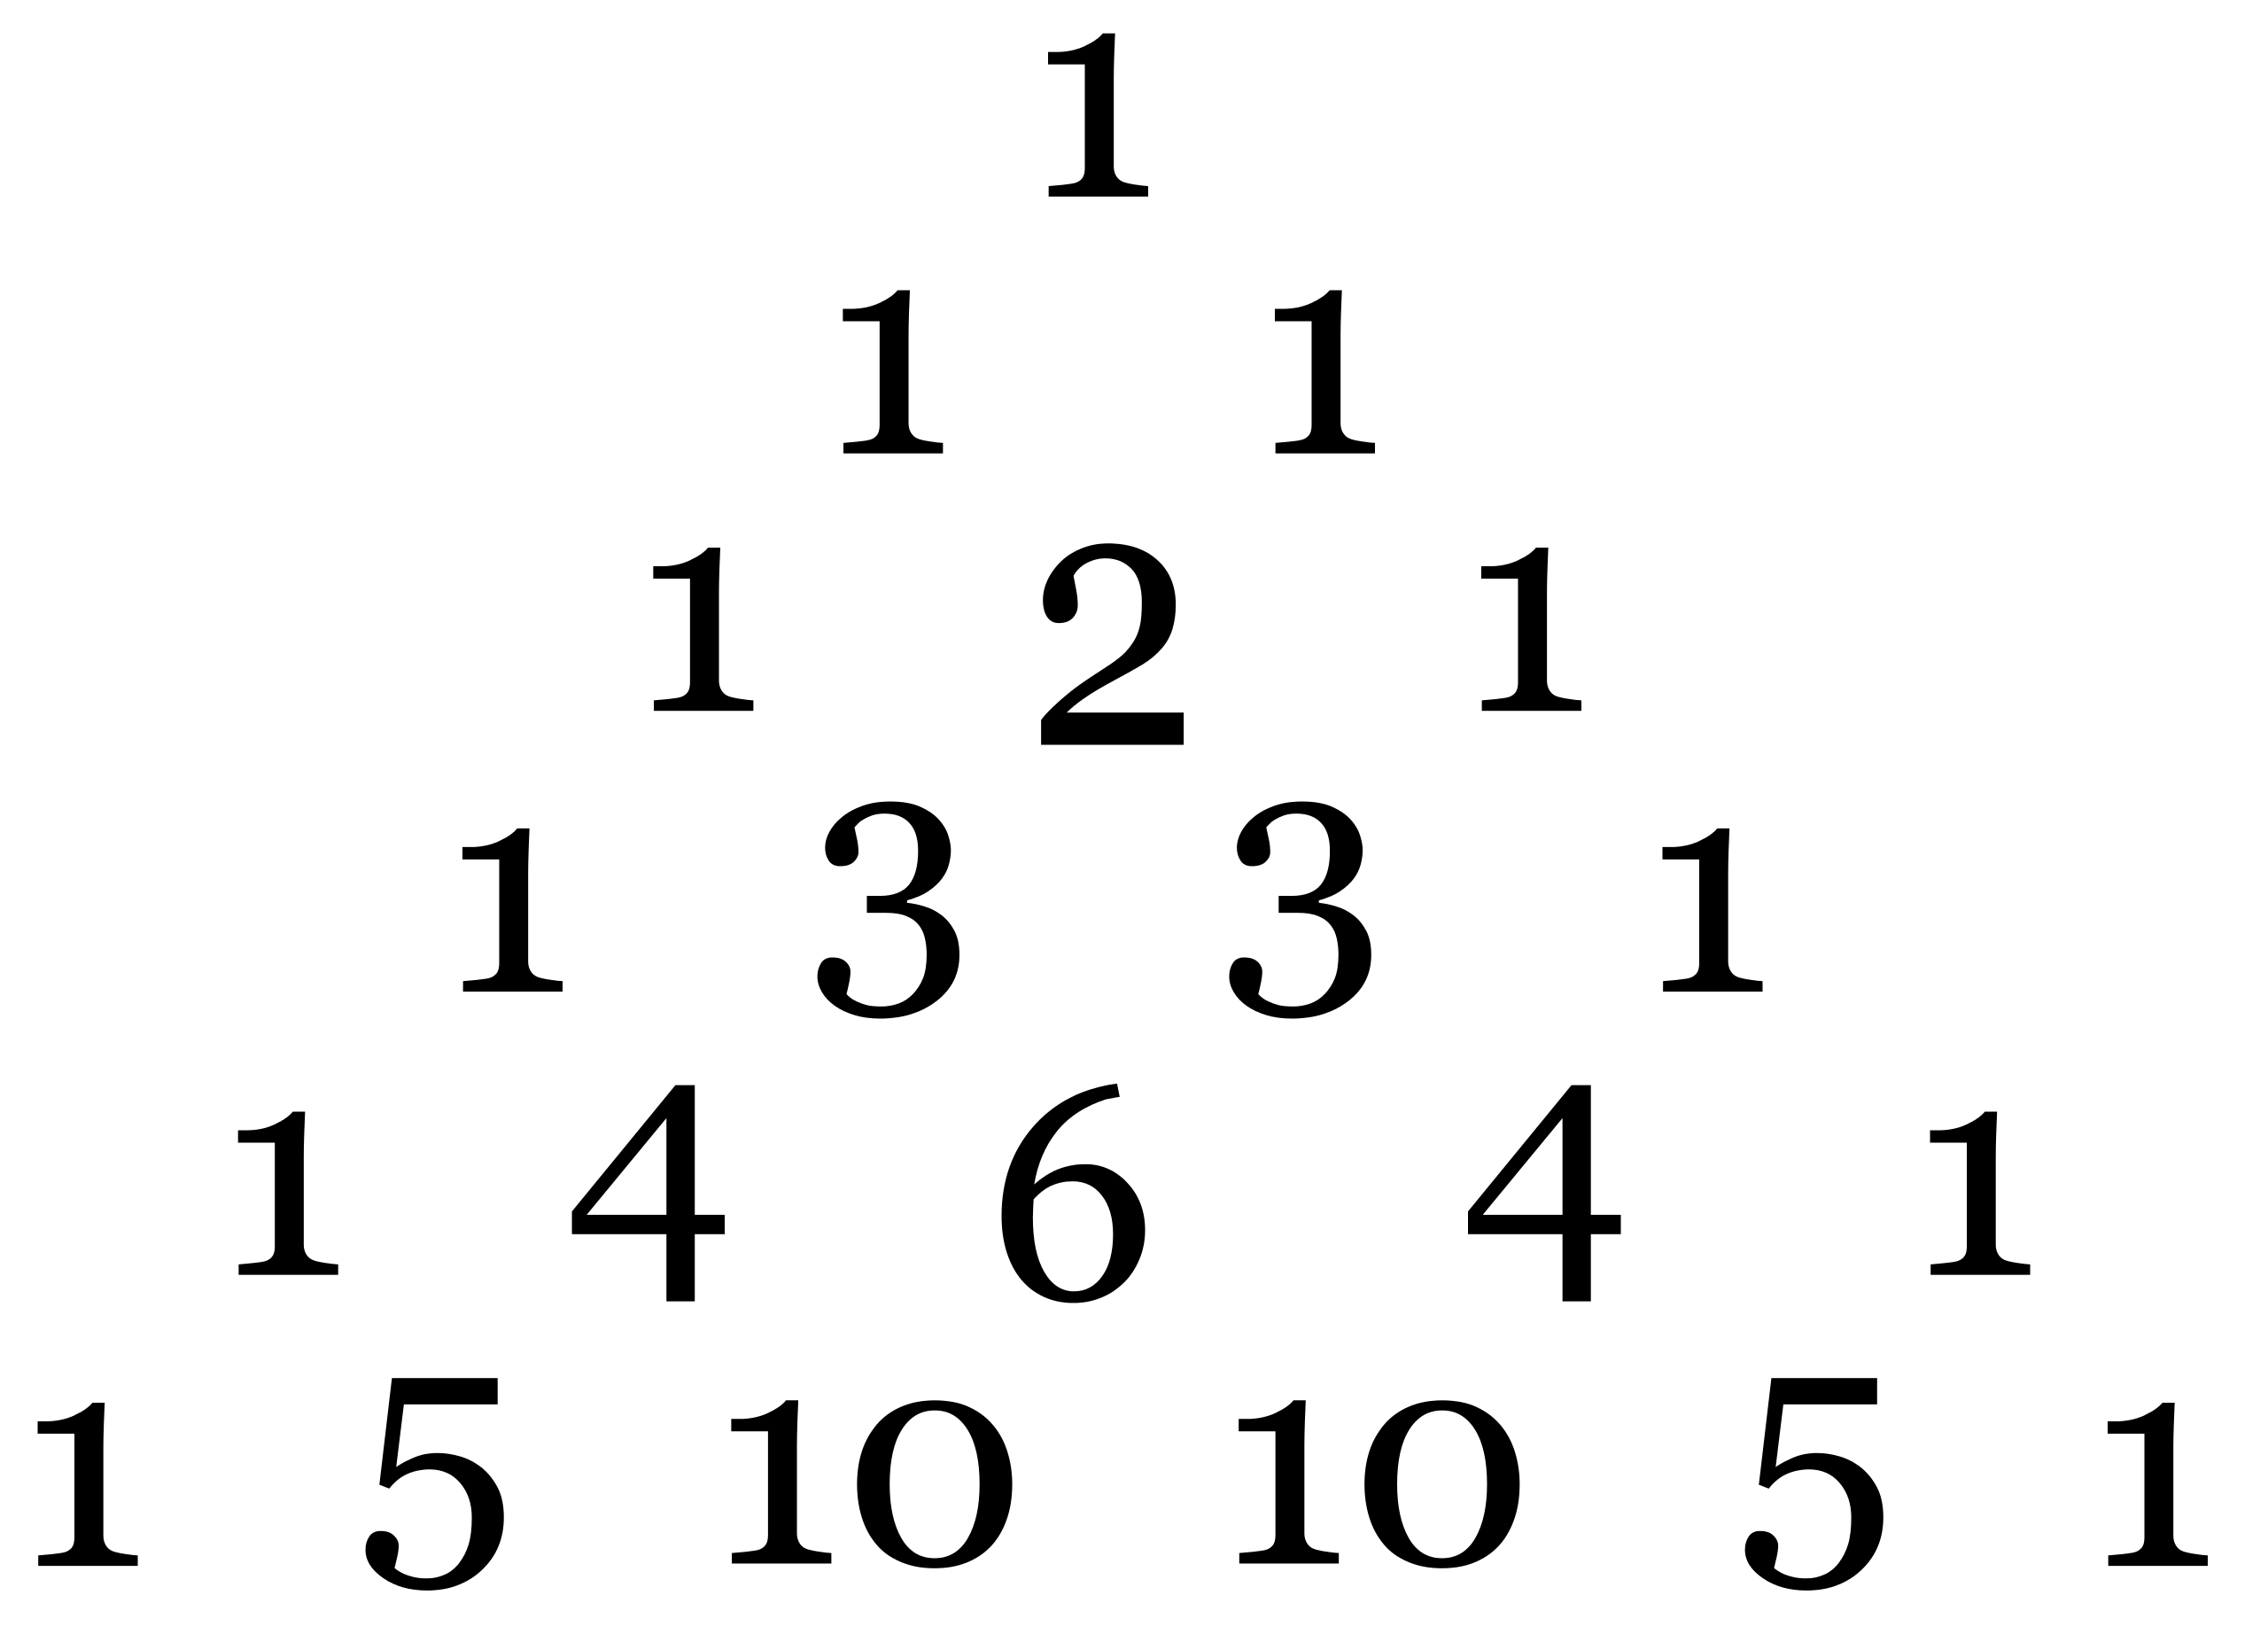
\includegraphics[width=0.4\linewidth]{src/images/pascals-triangle.png}
	\caption{杨辉三角形(又名帕斯卡三角形)}
	\label{fig:pascals-triangle}
\end{figure}

\subsection{应用}
熟练掌握组合数的性质和二项式展开的通项公式,可以解决大部分问题。对于另外一些问题,我们说不定还要深究二项式展开的根本思想。

\begin{example}
	已知$(\sqrt{x}-\frac{3}{x})^n$展开式只有第$5$项的二项式系数最大,求

	\begin{enumerate}
		\item $n$的值
		\item 展开式中$x^{-2}$的系数
		\item 所有有理项
	\end{enumerate}
\end{example}

\begin{proof}[解小题$1$]
	要第5项最大,根据组合数的性质得该数一定位于数列中央,故一共有9项,得$n=8$。
\end{proof}

\begin{proof}[解小题$2$]
	我们要先求出通项公式\[T_{r+1}=C_8^r(\sqrt{x})^{8-r}(-\frac{3}{x})^r=C_8^r(-3)^rx^{4-\frac{3}{2}r}\]

	使$x$的指数处等于$-2$,得\[4-\frac{3}{2}r=-2\Rightarrow r=4\]

	回代到通项公式得\[a=C_8^4(-3)^4=5670\qedhere\]
\end{proof}

\begin{proof}[解小题$3$]
	有理项即$x$的次数为整数的项,通过对通项公式中的$r$从0到8进行赋值,我们不难得出有如下5个有理项
	\begin{gather*}
		T_1=x^4\quad T_3=252x\quad T_5=5670x^{-2} \\
		T_7=20412x^{-5}\quad T_9=6561x^{-8} \qedhere
	\end{gather*}
\end{proof}

\begin{example}
	求$(a-2b+3c)^{10}$展开式中$a^2b^3c^5$的系数.
\end{example}

\begin{proof}[解]
	对于这种多项式问题,我们现在还没有方法可以将其直接展开。不过,千万不要忘记这不是一个代数问题,而是一个排列组合的问题呦!

	我们可以将它看成10个$a-2b+3c$相乘,要想构造$a^2b^3c^5$项,那么就要在10项中选2项拿出$a$,剩下的8项中选3项拿出$b$,以此类推。

	所以,我们可以算出展开式中$a^2b^3c^5$的系数是(不要忘记乘上原来的系数呦)\[C_{10}^2C_8^3C_5^5\times(-2)^3\times3^5=-4898880 \qedhere\]
\end{proof}

\section[多项式问题]{用赋值法解决多项式问题}
对于一个多项式$(x+a)^n$,已知其展开式为\[a_0+a_1x+a_2x^2+\cdots+a_nx^n\]我们就可以依据展开式给$x$赋值直接或间接地求出一些系数的线性组合的值。

如果我们要求常数项的值,可令$x$为0;求各项系数之和,则令$x$为1。

\begin{example}
	已知$(3x-1)^8=a_0+a_1x+a_2x^2+\cdots+a_8x^8$,求

	\begin{enumerate}
		\item 求各项系数之和
		\item 求各二项式系数之和
		\item 求$a_0-a_1+a_2-\cdots+a_8$
		\item 求$a_0+a_2+\cdots+a_8$
		\item 求$a_1+a_3+\cdots+a_7$
		\item 求$\dfrac{a_1}{2}+\dfrac{a_2}{4}+\cdots+\dfrac{a_8}{2^8}$
	\end{enumerate}
\end{example}

\begin{proof}[解小题$1$]
	通过观察展开式,不难发现只要令$x=1$即可
\end{proof}


	\part{概率和统计}
	\chapter{统计}

\section{统计图表}
\subsection{频率分布直方图}
\subsection{频率分布折线图}
\subsection{散点图}

\section{统计量}
在之前,我们已经学过了用均值和方差等统计量来估计总体的数字特征。现在,我们将复习已学的统计量并引入新的统计量。

\subsection{均值}
由于要表示大量数据的加法,我们引入求和符号$\Sigma$(读作sigma),${\displaystyle\sum_{i=0}^n a_i}$表示$a$从下标$i=0$到$i=n$的累加。

故此,均值公式可表示为
\begin{gather}
	\bar{x}=\frac{1}{n}\sum_{i=0}^n x_i \label{equ:mean-1}
\end{gather}

\subsection{方差和标准差}
\subsection{中位数和众数}
\subsection{百分位数}
\subsection{随机变量的分布特征}

\end{document}
